\documentclass[a4paper,12pt]{article}
\usepackage{graphicx}
\usepackage[backend=biber]{biblatex}
\usepackage{float}
\usepackage[swedish]{babel}
\usepackage{pdfpages} 
\usepackage[titletoc]{appendix}
\addbibresource{bibliography.bib}
%% Definitioner f�r LIPS-dokument

\usepackage[utf8]{inputenc}
\usepackage[swedish]{babel}
\usepackage[T1]{fontenc}
\usepackage{times}
\usepackage{ifthen}

\usepackage[margin=25mm]{geometry}

\usepackage{fancyhdr}
\pagestyle{fancy}
\lhead{}
\chead{\textbf{\LIPSprojekttitel}}
\rhead{\textbf{\LIPSdatum}}
\lfoot{\textbf{\LIPSkursnamn}\\\textbf{LIPS Slutrapport}}
\cfoot{\textbf{\thepage}\\\textbf{\LIPSgruppepost}}
\rfoot{\textbf{\LIPSprojektgrupp}}

\setlength{\parindent}{0pt}
\setlength{\parskip}{1ex plus 0.5ex minus 0.2ex}


\newcommand{\twodigit}[1]{\ifthenelse{#1<10}{0}{}{#1}}
\newcommand{\dagensdatum}{\number\year-\twodigit{\number\month}-\twodigit{\number\day}}

%%  Redefinitions of commands containing @
\makeatletter
\makeatother

\newcommand{\LIPStitelsida}{%
{\ }\vspace{45mm}
\begin{center}
  \textbf{\Huge \LIPSdokumenttyp}
\end{center}
\begin{center}
  {\Large Redaktör: \LIPSredaktor}
\end{center}
\begin{center}
  {\Large \textbf{Version \LIPSversion}}
\end{center}
\vfill
\begin{center}
  {\large Status}\\[1.5ex]
  \begin{tabular}{|*{3}{p{40mm}|}}
    \hline
    Granskad & \LIPSgranskare & \LIPSgranskatdatum \\
    \hline
    Godkänd & \LIPSgodkannare & \LIPSgodkantdatum \\
    \hline
  \end{tabular}
\end{center}
\newpage
}


\newenvironment{LIPSprojektidentitet}{%
{\ }\vspace{45mm}
\begin{center}
  {\Large PROJEKTIDENTITET}\\[0.5ex]
  {\small
  \LIPSartaltermin, \LIPSprojektgrupp\\
  Linköpings Tekniska Högskola, IFM
  }
\end{center}
\begin{center}
  {\small Gruppdeltagare}\\
%  \begin{tabular}{|p{30mm}|p{40mm}|p{35mm}|p{45mm}|}
  \begin{tabular}{|l|l|p{25mm}|l|}
    \hline
    \textbf{Namn} & \textbf{Ansvar} & \textbf{Telefon} & \textbf{E-post} \\
    \hline
}%
{%
    \hline
  \end{tabular}
\end{center}
\begin{center}
  {\small
    %\textbf{E-postlista för hela gruppen}: \LIPSgruppepost\\
    %\textbf{Hemsida}: \LIPSgrupphemsida\\[1ex]
    \textbf{Kund}: \LIPSkund\\
    \textbf{Kontaktperson hos kund}: \LIPSkundkontakt\\
    \textbf{Kursansvarig}: \LIPSkursansvarig\\
    \textbf{Handledare}: \LIPShandledare\\
  }
\end{center}
\newpage
}
\newcommand{\LIPSgruppmedlem}[4]{\hline {#1} & {#2} & {#3} & {#4} \\}



\newenvironment{LIPSdokumenthistorik}{%
\begin{center}
  Dokumenthistorik\\[1ex]
  \begin{small}
    \begin{tabular}{|l|l|p{60mm}|l|l|}
      \hline
      \textbf{Version} & \textbf{Datum} & \textbf{Utförda förändringar} & \textbf{Utförda av} & \textbf{Granskad} \\
      }%
    {%
      \hline
    \end{tabular}
  \end{small}
\end{center}
}
\newcommand{\LIPSversionsinfo}[5]{\hline {#1} & {#2} & {#3} & {#4} & {#5} \\}

\newcounter{LIPSkravnummer}
\newcounter{LIPSunderkravnummer}[LIPSkravnummer]
\newenvironment{LIPSkravlista}{%
  \begin{tabular}{|p{25mm}|p{25mm}|p{72mm}|p{18mm}|}
    }%
  {%
    \hline
  \end{tabular}
}
\newcommand{\LIPSkrav}[3]{\hline\stepcounter{LIPSkravnummer}\textbf{Krav nr \arabic{LIPSkravnummer}} & \textbf{{#1}} & {#2} & \textbf{{#3}} \\}
\newcommand{\LIPSunderkrav}[3]{\hline\stepcounter{LIPSunderkravnummer}\textbf{Krav nr \arabic{LIPSkravnummer}\Alph{LIPSunderkravnummer}} & \textbf{{#1}} & {#2} & \textbf{{#3}} \\}

\newcounter{LIPSMilstolpar}
\newenvironment{LIPSMilstolpslista}{%
  \begin{tabular}{|p{15mm}|p{72mm}|p{25mm}|}
\hline
\textbf{Nr} & \textbf{Beskrivning} & \textbf{Datum} \\
    }%
  {%
  \hline
  \end{tabular}
}
\newcommand{\LIPSMilstolpar}[2]{\hline\stepcounter{LIPSMilstolpar}\textbf{ \arabic{LIPSMilstolpar}.} & \textbf{{#1}} & \textbf{{#2}} \\}

\newcounter{LIPSBeslutspunkter}
\newenvironment{LIPSBeslutspunktslista}{%
  \begin{tabular}{|p{15mm}|p{72mm}|p{25mm}|}
\hline
\textbf{Nr} & \textbf{Beskrivning} & \textbf{Datum} \\
    }%
  {%
  \hline
  \end{tabular}
}
\setcounter{LIPSBeslutspunkter}{-1}
\newcommand{\LIPSBeslutspunkter}[2]{\hline\stepcounter{LIPSBeslutspunkter}\textbf{ \arabic{LIPSBeslutspunkter}.} & \textbf{{#1}} & \textbf{{#2}} \\}

\newcounter{LIPSAktiviteter}
\newenvironment{LIPSAktivitetslista}{%
  \begin{tabular}{|p{15mm}|p{72mm}|p{25mm}|}
\hline
\textbf{Nr} & \textbf{Beskrivning} & \textbf{Datum} \\
    }%
  {%
  \hline
  \end{tabular}
}
\newcommand{\LIPSAktiviteter}[2]{\hline\stepcounter{LIPSAktiviteter}\textbf{ \arabic{LIPSAktiviteter}.} & \textbf{{#1}} & \textbf{{#2}} \\}




%%% Local Variables: 
%%% mode: latex
%%% TeX-master: "kravspec_mall"
%%% End: 
\pagenumbering{roman}
\newcommand{\LIPSartaltermin}{2018/VT}
\newcommand{\LIPSkursnamn}{TFYA75}

\newcommand{\LIPSprojekttitel}{Visualisering av elektronstruktur}

\newcommand{\LIPSprojektgrupp}{Grupp 2}
\newcommand{\LIPSgruppepost}{}
\newcommand{\LIPSdokumentansvarig}{Marian Brännvall}

\newcommand{\LIPSkund}{IFM, Linköpings universitet, 581\,83 Linköping}
\newcommand{\LIPSkundkontakt}{Rickard Armiento, 013-281249, rickard.armiento@liu.se}
\newcommand{\LIPSkursansvarig}{Per Sandström, 013-282902, persa@ifm.liu.se}
\newcommand{\LIPShandledare}{Johan Jönsson, 013-281176, johan.jonsson@liu.se}


\newcommand{\LIPSdokumenttyp}{Kappa}
\newcommand{\LIPSredaktor}{Anders Rehult}
\newcommand{\LIPSversion}{xx}
\newcommand{\LIPSdatum}{\dagensdatum}

\newcommand{\LIPSgranskare}{DOK}
\newcommand{\LIPSgranskatdatum}{18-03-05}
\newcommand{\LIPSgodkannare}{}
\newcommand{\LIPSgodkantdatum}{}

\usepackage[titletoc]{appendix}
\usepackage{hyperref}
\hypersetup{
    colorlinks,
    citecolor=black,
    filecolor=black,
    linkcolor=black,
    urlcolor=black
}

\begin{document}

\LIPStitelsida

\begin{LIPSprojektidentitet}
  \LIPSgruppmedlem{Anders Rehult}{Projektledare (PL)}{076-3161206}{andre449@student.liu.se}
  \LIPSgruppmedlem{\LIPSdokumentansvarig}{Dokumentansvarig (DOK)}{070-7280044}{marbr639@student.liu.se}
  \LIPSgruppmedlem{Andreas Kempe}{Sekreterare (SE)}{073-9796689}{andke133@student.liu.se}
  \LIPSgruppmedlem{Viktor Bernholtz}{Viktor Bernholtz (VB)}{073-0386030}{vikbe253@student.liu.se}
\end{LIPSprojektidentitet}

\tableofcontents{}
\newpage

\addcontentsline{toc}{section}{Dokumenthistorik}
\begin{LIPSdokumenthistorik}
  \LIPSversionsinfo{0.1}{2018-02-27}{Första utkast.}{Projektgruppen}{SE}
    \LIPSversionsinfo{0.2}{2018-03-05}{Andra utkast.}{Projektgruppen}{DOK}
\end{LIPSdokumenthistorik}
\newpage
\pagenumbering{arabic}

\section{Inledning}
Dokumentet är en kappa för kandidatprojektet i visualisering av elektronstrukturer. Visualisering av elektronstrukturer är ett av projekten i kursen TFYA75 vid
Linköpings universitet. Kappan är en sammanfattning av hela projektet.

\subsection{Parter}
Rickard Armiento har beställt systemet som är beskrivet i kappan. Medlemmarna i projektgruppen, som är listade under rubriken projektidentitet ovan, är mottagare av denna beställning och har haft i uppgift att implementera systemet. Projektgruppens handledare är Johan Jönsson.

\subsection{Syfte och mål}
Inom materialfysik är elektronstrukturberäkningar ett viktigt teoretiskt verktyg. Detta för att få en så bra förståelse som möjligt av hur olika material är uppbyggda, bland annat vad gäller kristallers egenskaper sett ur ett kvantmekaniskt perspektiv. Det kan exempelvis handla om att man vill ta reda på olika materials egenskaper vad gäller värmeledningsförmåga, strömledningsförmåga etc.

För att öka förståelsen samt för att enklare kunna presentera resultat från forskning inom området är det viktigt att kunna göra olika typer av visualiseringar baserat på elektronstrukturberäkningar.

I många av de system som används för att utföra dessa beräkningar, exempelvis VASP, ges ingen eller begränsad möjlighet till detta. Vidare är de system som idag finns tillgängliga för visualisering förhållandevis ineffektiva, dåligt standardiserade samt har få visualiseringsfunktioner.

Syftet och målet för projektet har varit att uppdatera och utöka det modifierbara verktyg för visualisering av resultaten från elektronstrukturberäkningar som togs fram av 2017 års projektgrupp. Utöver det konkreta målet med utvecklingen av mjukvara för visualisering ska även projektet ge projektmedlemmarna erfarenhet av att arbeta i projekt och utöka deras förmåga till analytiskt och fysikaliskt tänkande för att ge värdefull erfarenhet inför arbetslivet.

\subsection{Användning}
Denna produkt kommer användas vid Linköpings universitet för att analysera data från elektronstruktursberäkningar.

\subsection{Begränsningar}
I projektet kommer visualiseringsverktyget Inviwo och
programmeringspråken Python och C++ användas. Det kommer inte utredas
om det är bättre att använda andra verktyg.

\subsection{Definitioner}

\textbf{C++} är ett programmeringsspråk.
\cite{C++}
\newline
I Inviwo används C++ för att skriva programkod till
processorer.

\textbf{Fermi-yta} är, för elektroners k-punkter i reciproka rymden, isoytan där elektronernas energi är lika med Fermi-energin.
\cite{Fermi-yta}

\textbf{HDF5} är ett filformat som kan hantera stora mängder data.
\cite{hdf5}

\textbf{Inviwo} (Interactive Visualization Workshop) är programvara
för visualisering som tillhandahåller en nätverksredigerare för
designen av dataflödesnätverk. Noderna i dessa dataflödesnätverk
kallas processorer. Indata till nätverket behandlas i dessa
processorer och utdata genereras.
\cite{Inviwo}

\textbf{Python} är ett programmeringsspråk.
\cite{Python}
\newline
I Inviwo används Python för att knyta samman processorer.

\section{Kunskapsbas}
\label{kunskapsbas}
Projektgruppen har efter att tagit del av projektdirektivet, se appendix \ref{appendix:projektdirektiv}
skrivit en kravspecifikation, se appendix \ref{appendix:kravspecifikation}. Därefter skrevs en projektplan, se appendix \ref{appendix:projektplan}, tidplan, se appendix \ref{appendix:tidplan} och en  systemskiss, se appendix \ref{appendix:systemskiss} enligt LIPS-modellen \cite{LIPS}. 
% TODO: Fixa ref för LIPS
Dessa dokument har sedan fungerat som en utgångspunkt för projektets utforming. Utöver dessa har en designspecifikation, se appendix \ref{appendix:designspecifikation} skrivits som är en fördjupning i systemskissen och ger en mer detaljerad beskrivning av systemet.

Projektgruppen har skrivit två fördjupningsarbeten, se appendix \ref{appendix:fermi-ytor} och \ref{appendix:visualisering} knutna till projektarbetet.

Utöver detta har projektgruppen haft ett antal föreläsningar och laborationer inom området.

\section{Fasplan}
Projektet drivs enligt LIPS-modellen, som är en modell med regler, instruktioner och mallar för att bedriva projekt. Projektet delas upp i tre faser - före, under, och efter.

\subsubsection{Före-fas}
Före-fasen är ämnad att undersöka om projektet bör genomföras och, om så är fallet, definiera och konkretisera projektets mål samt organisera arbetet som krävs för att uppnå dessa. Under före-fasen skrivs bland annat ett projektdirektiv, se appendix \ref{appendix:projektdirektiv}, en kravspecifikation, se appendix \ref{appendix:kravspecifikation}, en systemskiss, se appendix \ref{appendix:systemskiss} och en projektplan, se appendix \ref{appendix:projektplan}. Projektdirektivet skrevs innan projektgruppen skapades och gavs till projektgruppen vid projektets start.
Projektgruppen har under före-fasen skrivit ett gruppkontrakt, se appendix \ref{appendix:Gruppkontrakt}, en kravspecifikation, en systemskiss samt en projektplan.

\subsubsection{Under-fas}
Under  under-fasen  utförs  det  arbete  som  leder  till  att  projektets  krav  uppfylls.  Projektgrup-
pen skriver en designspecifikation, se appendix \ref{appendix:designspecifikation}
som beskriver hur systemet ska konstrueras i mer detalj än
systemskissen. Projektgruppen arbetar sedan med att, utgående från denna designspecifikation, konstruera och testa systemet. En teknisk dokumentation, se appendix \ref{appendix:teknisk-dokumentation}, skrivs parallellt med systemets konstruktion för att reflektera den faktiska implementationen av idéerna beskrivna i designspecifikationen. 

Projektgruppen har också skrivit två fördjupningsarbeten knutna till projektet. Det ena, se appendix \ref{appendix:fermi-ytor}, behandlar Fermi-ytor som är ett av fördjupningsområdena i projektet. Det andra, se appendix \ref{appendix:visualisering}, behandlar visualisering som är en mer generell del av projektet. 

\subsubsection{Efter-fas}
Under efter-fasen överförs projektresultatet till beställaren och projektet avslutas. Projektgruppen skriver en kappa som bifogas vid slutleveransen av produkten och även en användarmanual, se appendix \ref{appendix:användarmanual}. Vid slutleveransen ska
även en demonstration hållas som visar att produkten uppfyller kraven ställda på den. Efter produkten levererats skriver projektgruppen en efterstudie.

\section{Fördjupningsarbeten}
\label{ch:fordjupningsarbeten}
Nedan beskrivs kortfattat de fördjupningsarbeten som gjort under projektet. Dessa finns även i sin helhet i appendix \ref{appendix:fermi-ytor} och \ref{appendix:visualisering}. 
\subsection{Fermi-ytor}
Syftet med fördjupningsarbetet om Fermi-ytor var att besvara följande frågor: Vad är Fermi-ytor och hur kan dessa beräknas numeriskt. Detta var av intresse för projektet eftersom en del av det bestod i att visualisera Fermi-ytor...

\subsection{Visualisering av volymdata}

\section{Teknisk beskrivning}

En teknisk beskrivning av det  färdigställda systemet kan ses i figur \ref{fig:grov-skiss}. % lägg till fig
Systemet hanterar indata från VASP. %TODO: Lägg till om vi har elk
%och även från Elk.
Datan kommer från elektronstrukturberäkningar och konverteras till HDF5-format för att därefter visualiseras. Användaren kan välja vad som ska visualiseras, kontrollera renderingens utseende och ställa in egenskaper såsom färg, transparens och rotation.
Systemet har delats in i delsystem och dessa har utvecklas och testas enskilt i den mån det inte funnits beroenden till andra delsystem.

\begin{figure}[H]
	\centering
	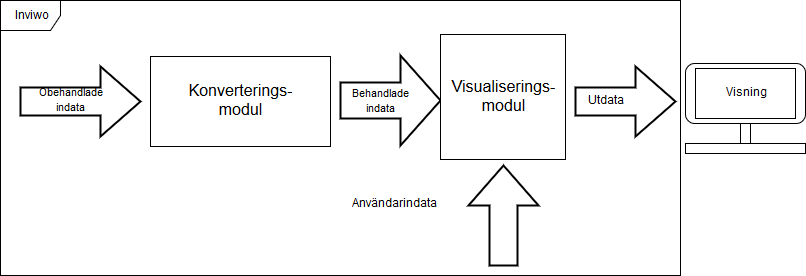
\includegraphics[scale=0.55]{grov-skiss.png}
	\caption{Grov design av systemet}
	\label{fig:grov-skiss}
\end{figure}

I avsnitt \ref{datakonvertering} och \ref{visualisering} nedan ges en övergripande inblick av det två stora delsystemen och deras delsystem. För en mer detaljerad teknisk beskriving av systemet se den tekniska dokumentationen, se appendix \ref{appendix:teknisk-dokumentation}.

\subsection{Datakonvertering}
\label{datakonvertering}
Detta avsnitt behandlar delsystemet datakonvertering, figur \ref{fig:konverteringdetalj} ger en grov översikt av delsystemet. Obehandlad data skickas in, obehandlad data är i form av textfiler med data från beräkningar gjorda i VASP.% TODO: Lägg till ELk om vi fixar det.
% eller Elk.
Indata behandlas sedan i konverteringsmodulen. Från konverteringsmodulen kommer behandlad data i HDF5-format.

\begin{figure}[H]
	\centering
	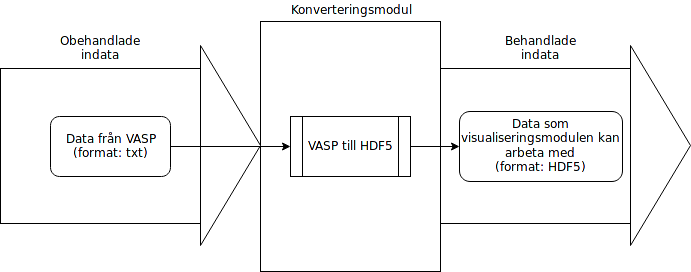
\includegraphics[scale=0.55]{konverteringdetalj.png}
	\caption{Grov design av konverteringsmodulen}
	\label{fig:konverteringdetalj}
\end{figure}

\subsubsection{HDF5}
Systemet kan hantera de olika utdatafilerna från VASP.%TODO: Lägg till elk om vi fixar det.
%Det bör även kunna hantera utdatafiler från Elk.
Detta görs genom att konvertera datan till HDF5-format.
HDF5 är ett filformat som är designat för att hantera stora mängder data på ett flexibelt sätt \cite{hdf5}.
HDF5 har flera olika datatyper, se Figur 3, och ett HDF5-objekt som antingen är lagrat på disk eller hålls i minnet är uppdelat i två huvudsakliga underobjekt, nämligen grupper och dataset.
%ref[8, s. 3-4]

Alla HDF5-objekt har en rotgrupp som äger alla andra objekt i datastrukturen. Denna grupp innehåller i sin tur all övrig data i form av andra grupper, länkar till andra grupper eller dataset.
Dataset innehåller rådata av något slag. Rådata kan i sammanhanget vara bilder, utdata från beräkningar, programdata, etcetera. %ref [8, s. 4-5]
I desingspesifikationen, se appendix \ref{appendix:designspecifikation} ges en mer detaljerad beskriving av HDF5.

\subsubsection{VASP}
Från beräkningsprogrammet VASP fås en rad olika utdatafiler. Dessa listas och beskrivs i designspecifikationen %tekniska dokumentationen?
(se appendix X). Ur dessa utdatafiler läses saker som atompositionsdata, gittervektorer, elektrontäthetsdata, tillståndstäthetsdata, Fermi-energi och så vidare för att kunna visualisera kristallstrukturer, elektrontäthet, ELF, tillståndstäthet och Fermi-ytor. I designspecifikationen %tekniska dokumentationen?
beskrivs närmare vad som läses från vilka utdata filer. 
%TODO: Lägg till Elk om vi fixar det.
%\subsubsection{ELK}

\subsection{Visualisering}
Figur \ref{fig:visualisering} visar hur delsystemet Visualisering är uppbyggt. Behandlad samt användarindata skickas in. Användarindata består av val av färg, val av egenskap som ska ritas ut, val av transparens etc. Dessa behandlas sedan i visualiseringsmodulen som skapar en bild utifrån dem. Den utritade bilden skickas sedan ut från modulen. Detta är en allmän beskrivning av visualiseringen, för de olika egenskaperna som visualiseras är mittenrektangeln i Figur \ref{fig:visualisering} uppbyggd på olika sätt med olika processorer.
\label{visualisering}
\begin{figure}[H]
	\centering
	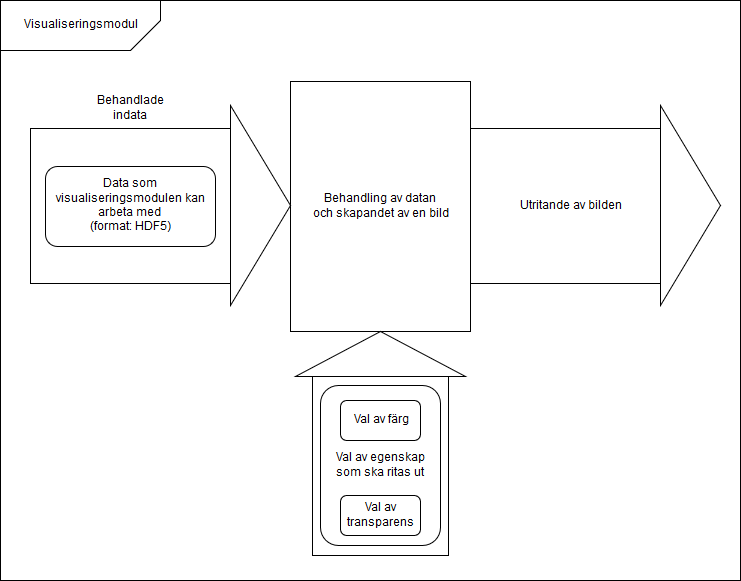
\includegraphics[scale=0.55]{Visualisering.png}
	\caption{Grov design av delsystemet Visualisering}
	\label{fig:visualisering}
\end{figure}
\subsubsection{Utriting}
Delsystemet ritar ut bilder utefter den behandlade datan. Utritningen ger en visualisering av den egenskap som modulen behandlar och kan till exempel vara en volymrendering eller en 2D-graf, beroende på vilket som är mest lättolkat. 

Utritningen görs via Inviwos inbyggda funktionalitet för att rendera via OpenGL. 
\subsubsection{Användarindata}
% TODO: Fixa nya figurer från inviwo
Användaren kan ändra inställningar som kontrollerar utseendet på visualiseringarna.
Denna indata matas in i Inviwos användargränssnitt, %fixa fig
se Figur 10, och i inställningsrutan för en processor, %fixa fig
se Figur 11.
Visualiseringsfunktionaliteten läggas till i form av processorer som via Inviwo tillhandahåller inställningsmöjligheter på det sätt som beskrivits i designspecifikationen \ref{appendix:designspecifikation}. Således blir inte användarinställningar ett eget separat delsystem, utan kommer att bakas in i visualiseringssystemen. Detta görs genom att processorerna är skrivna att exponera de inställningar som användaren är menad att
justera. Inviwo kommer då automatiskt lägga till inställningarna i rutan, se %fixa figur 
Figur 11.

\subsubsection{Interaktivitet}
Användaren kan modifiera visualiseringen genom att reglera ett intervall av värden för
någon egenskap, där full transparens fås för alla värden inom intervallet, rotera 3D-bilder etc.
Ny användarindata, som skickas in efter att den första bilden har ritats upp, skickas tillbaka till
visualiseringsmodulen för att utföra en ny rendering.
% TODO: Lägg till exempel med bild?

\subsubsection{Kristallstruktur}
Kristallstruktur kan visualiseras som atompositioner i enhetscellen. Sfärer som representerar atomer  kan  ritas  ut  genom  volymsrendering. % figur och exempel?
I designspecifikationen, se appendix \ref{appendix:designspecifikation} för en mer detaljerad beskrivning
hur detta byggs upp.
% TODO: Lägg till exempel med bild?

\subsubsection{Elektrontäthet}
Elektrontäthet kan visualiseras genom volymsrendering. Det är alltså sannolikheten för att hitta elektronener på olika positioner som visualiseras. Se figur %figur och exempel?
I designspecifikationen, se appendix \ref{appendix:designspecifikation} för en mer detaljerad beskrivning av elektrontäthet.
% TODO: Lägg till exempel med bild?

\subsubsection{Tillståndstäthet}
Tillståndstäthet kan visualiseras med en 2D-graf med energn på x-axeln och tillståndstätheten på y-axeln.. se figur %figur och exempel?
I designspecifikationen, se appendix \ref{appendix:designspecifikation} för e mer detaljerad besrivning av tillståndstäthet.

\subsubsection{Fermi-ytor}

\subsubsection{Dynamisk visualisering av kristallstrukturer}



\section{Resultat}

\section{Slutsats}



\newpage
\addcontentsline{toc}{section}{Referenser}
\printbibliography{}

\begin{appendices}

\section{Användarmanual}
\label{appendix:användarmanual}	
	
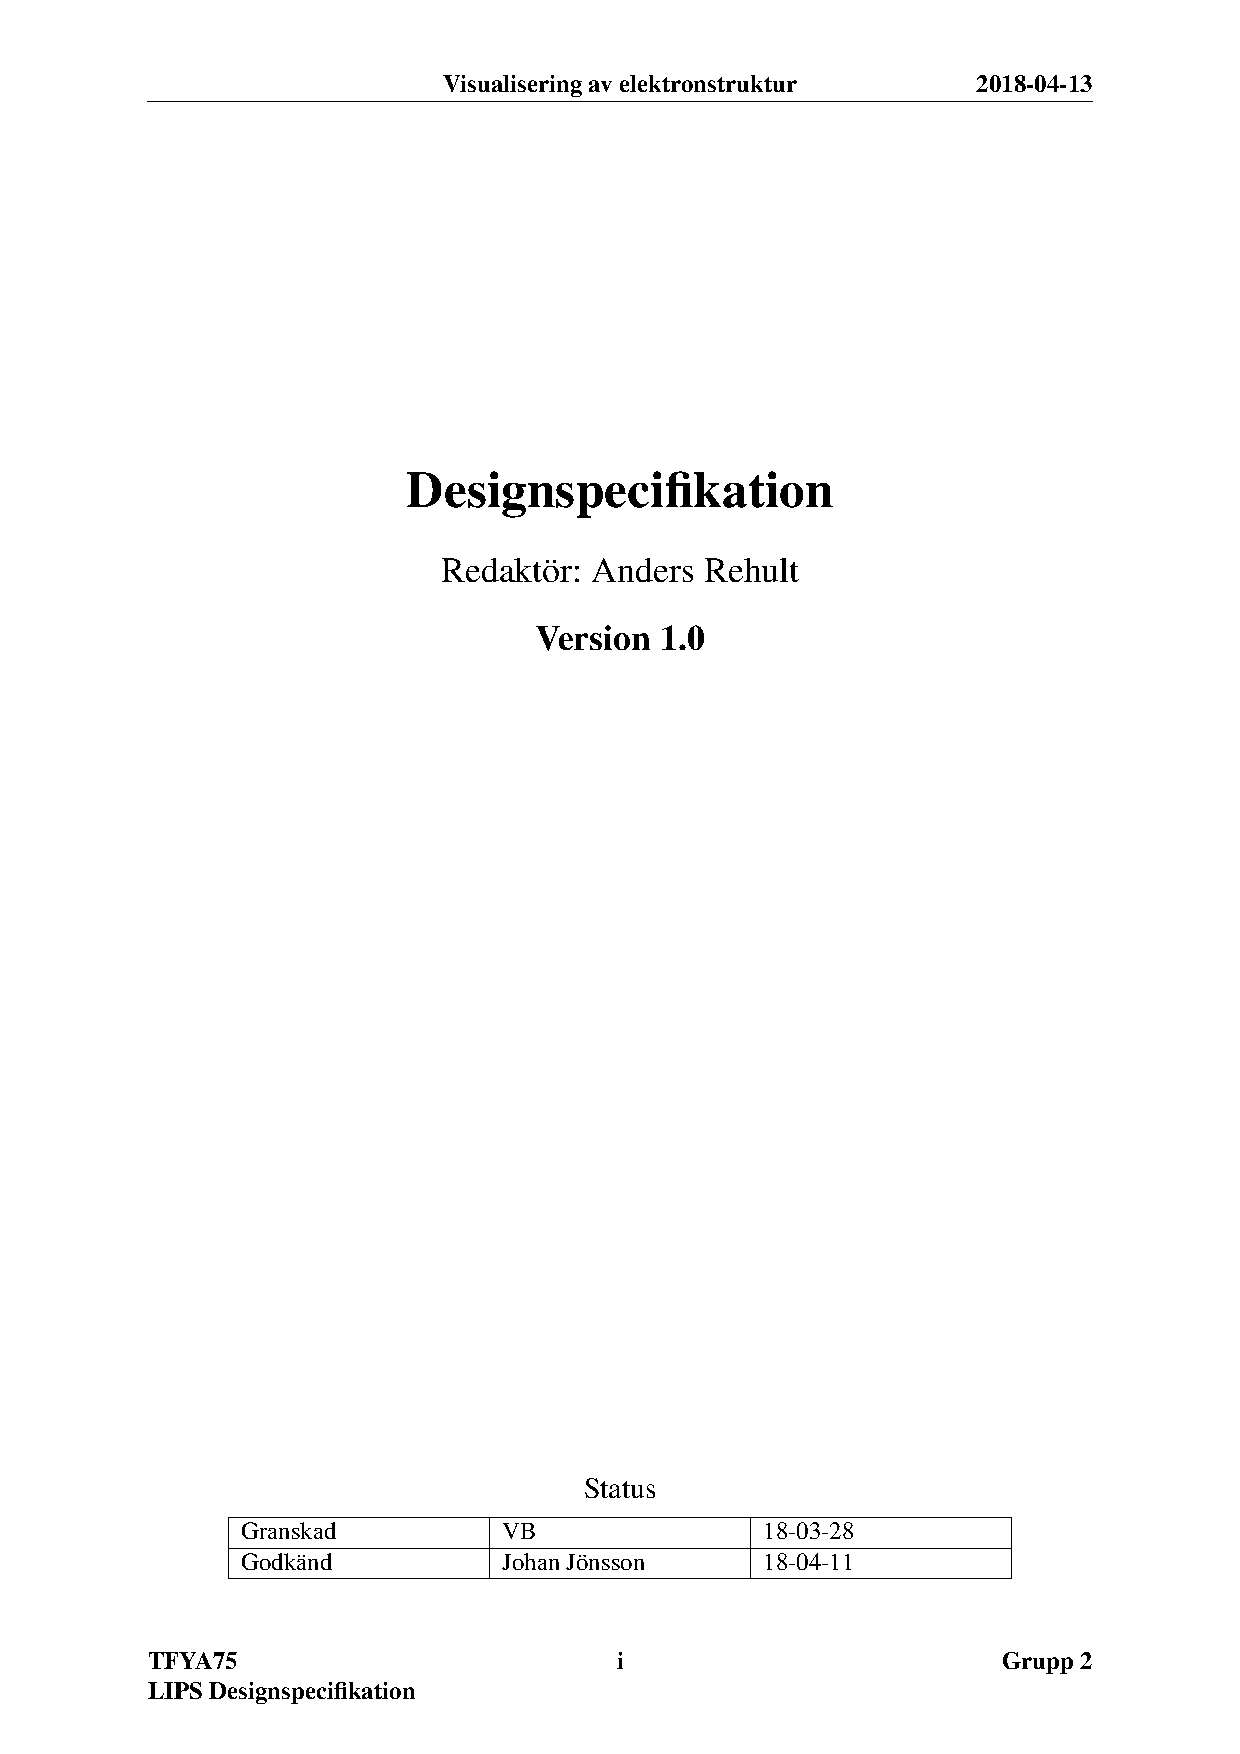
\includepdf[pages={1},pagecommand=\section{Designspecifikation}\label{appendix:designspecifikation}\thispagestyle{empty}]{designspecifikation_10.pdf} \includepdf[pages={2-}]{designspecifikation_10.pdf}
	
	
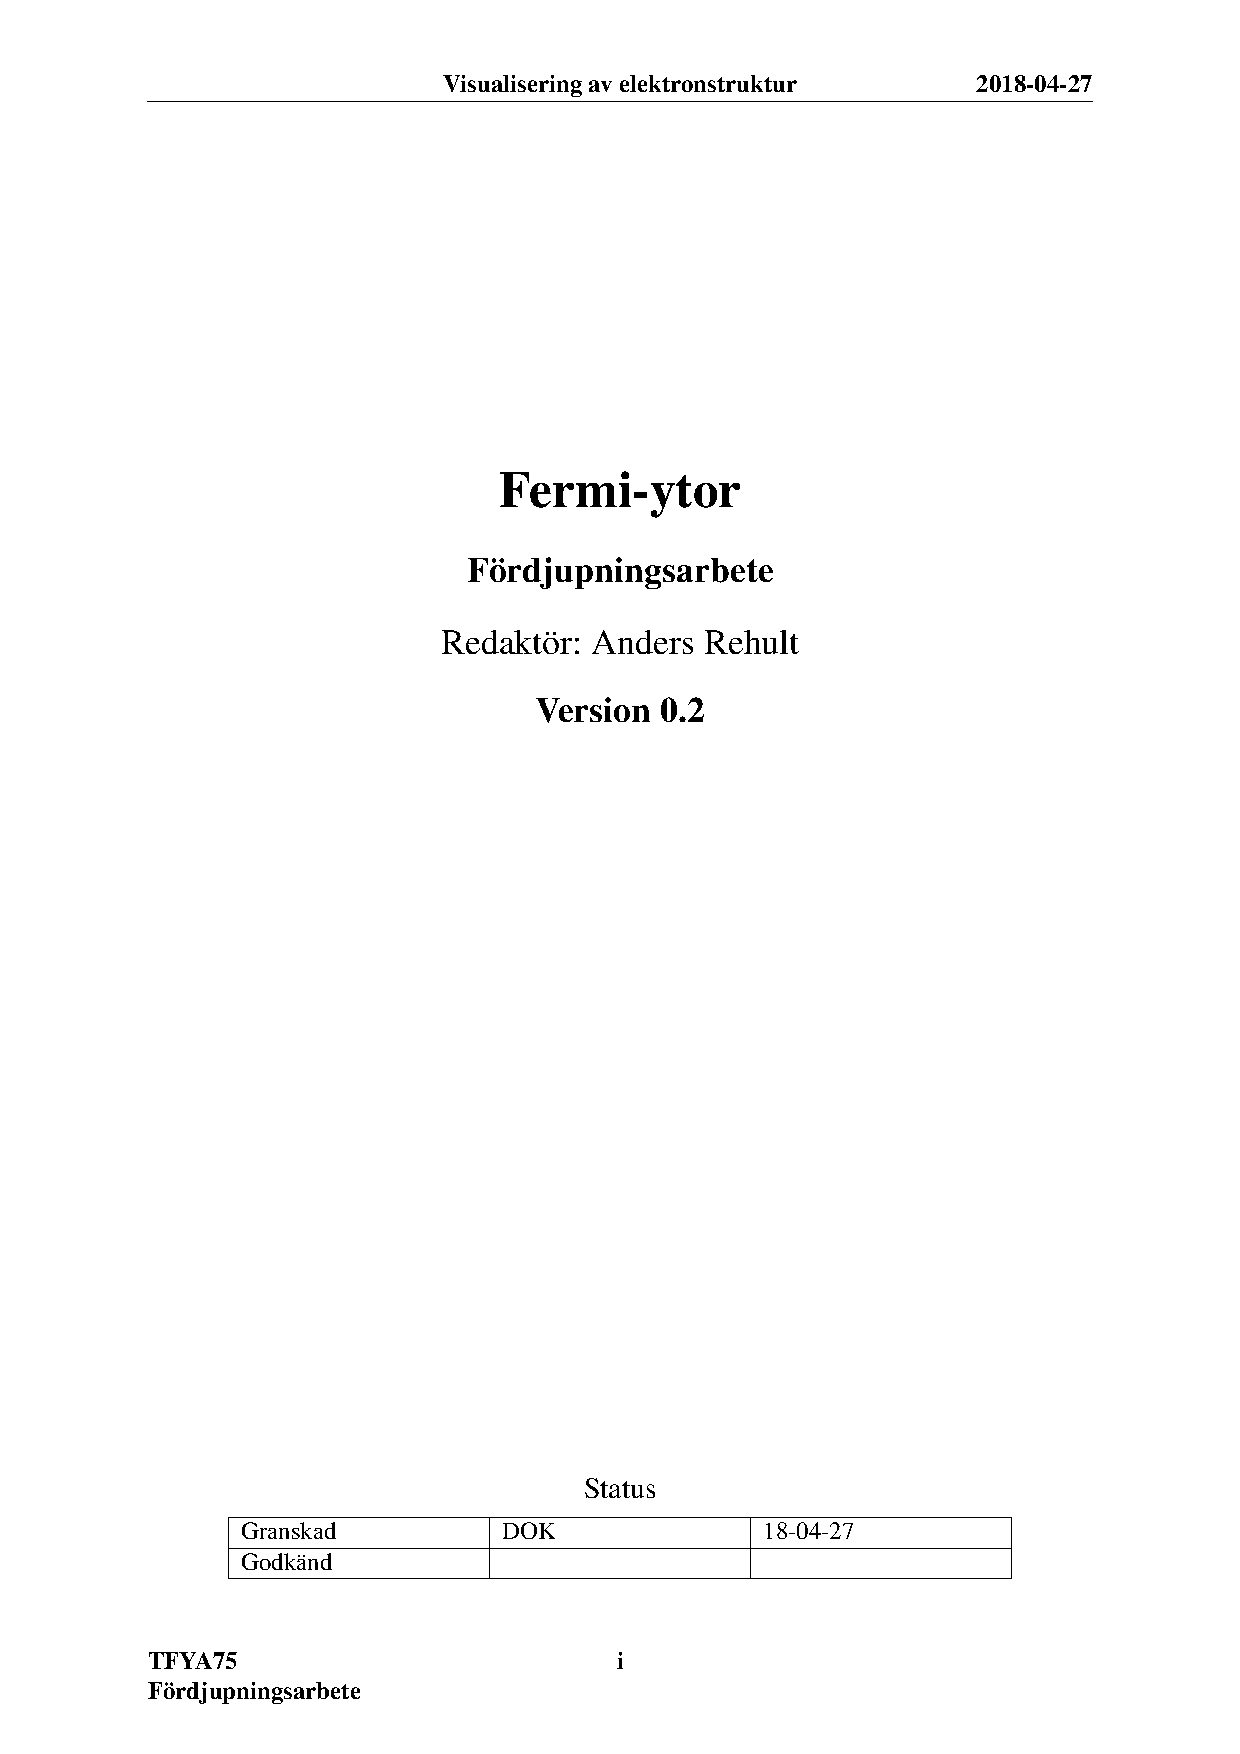
\includepdf[pages={1},pagecommand=\section{Fördjupningsarbete - Fermi-ytor }\label{appendix:fermi-ytor}\thispagestyle{empty}]{fordjupningsarbete-fermi-ytor_02.pdf}
\includepdf[pages={2-}]{fordjupningsarbete-fermi-ytor_02.pdf}

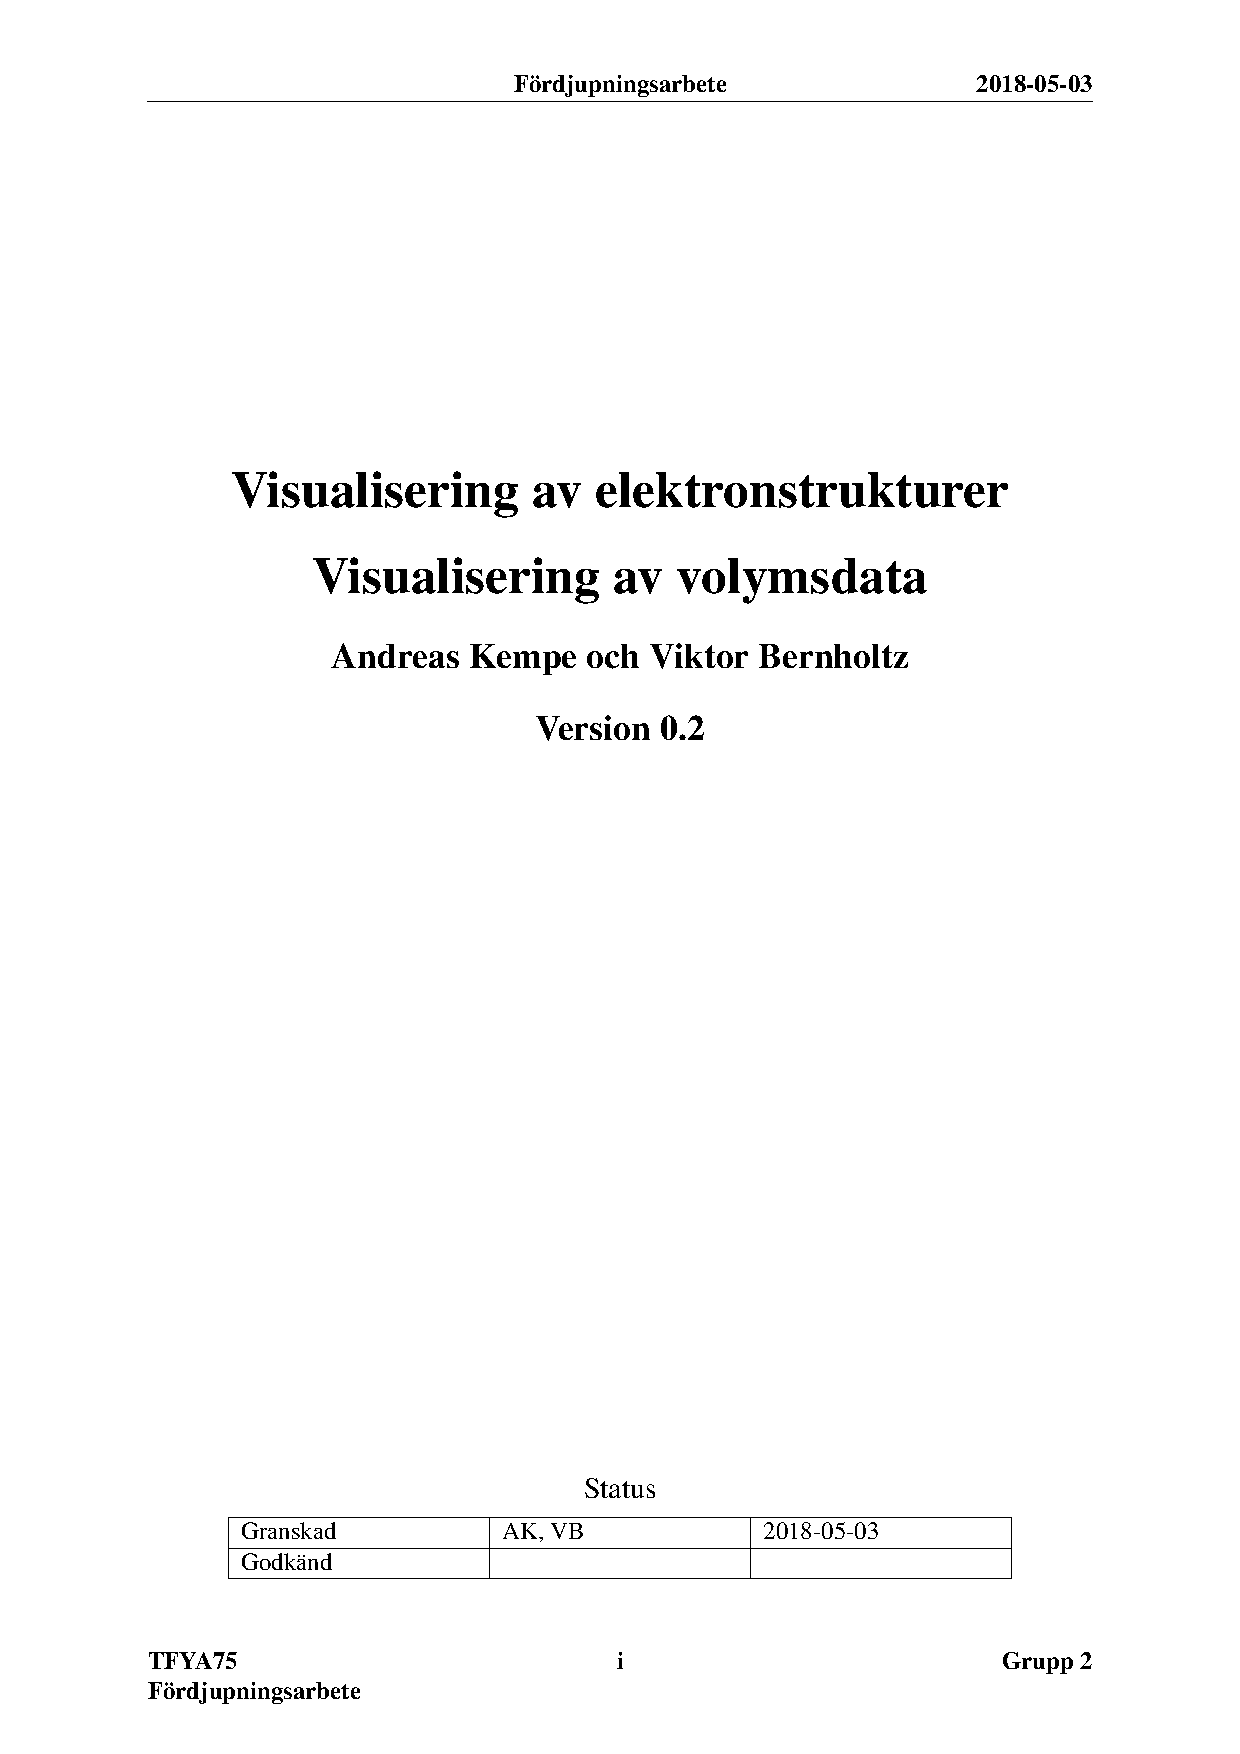
\includepdf[pages={1},pagecommand=\section{Fördjupningsarbete - Visualisering av volysmdata}\label{appendix:visualisering}\thispagestyle{empty}]{Visualisering-av-volymsdata_02.pdf}
\includepdf[pages={2-}]{Visualisering-av-volymsdata_02.pdf}
	
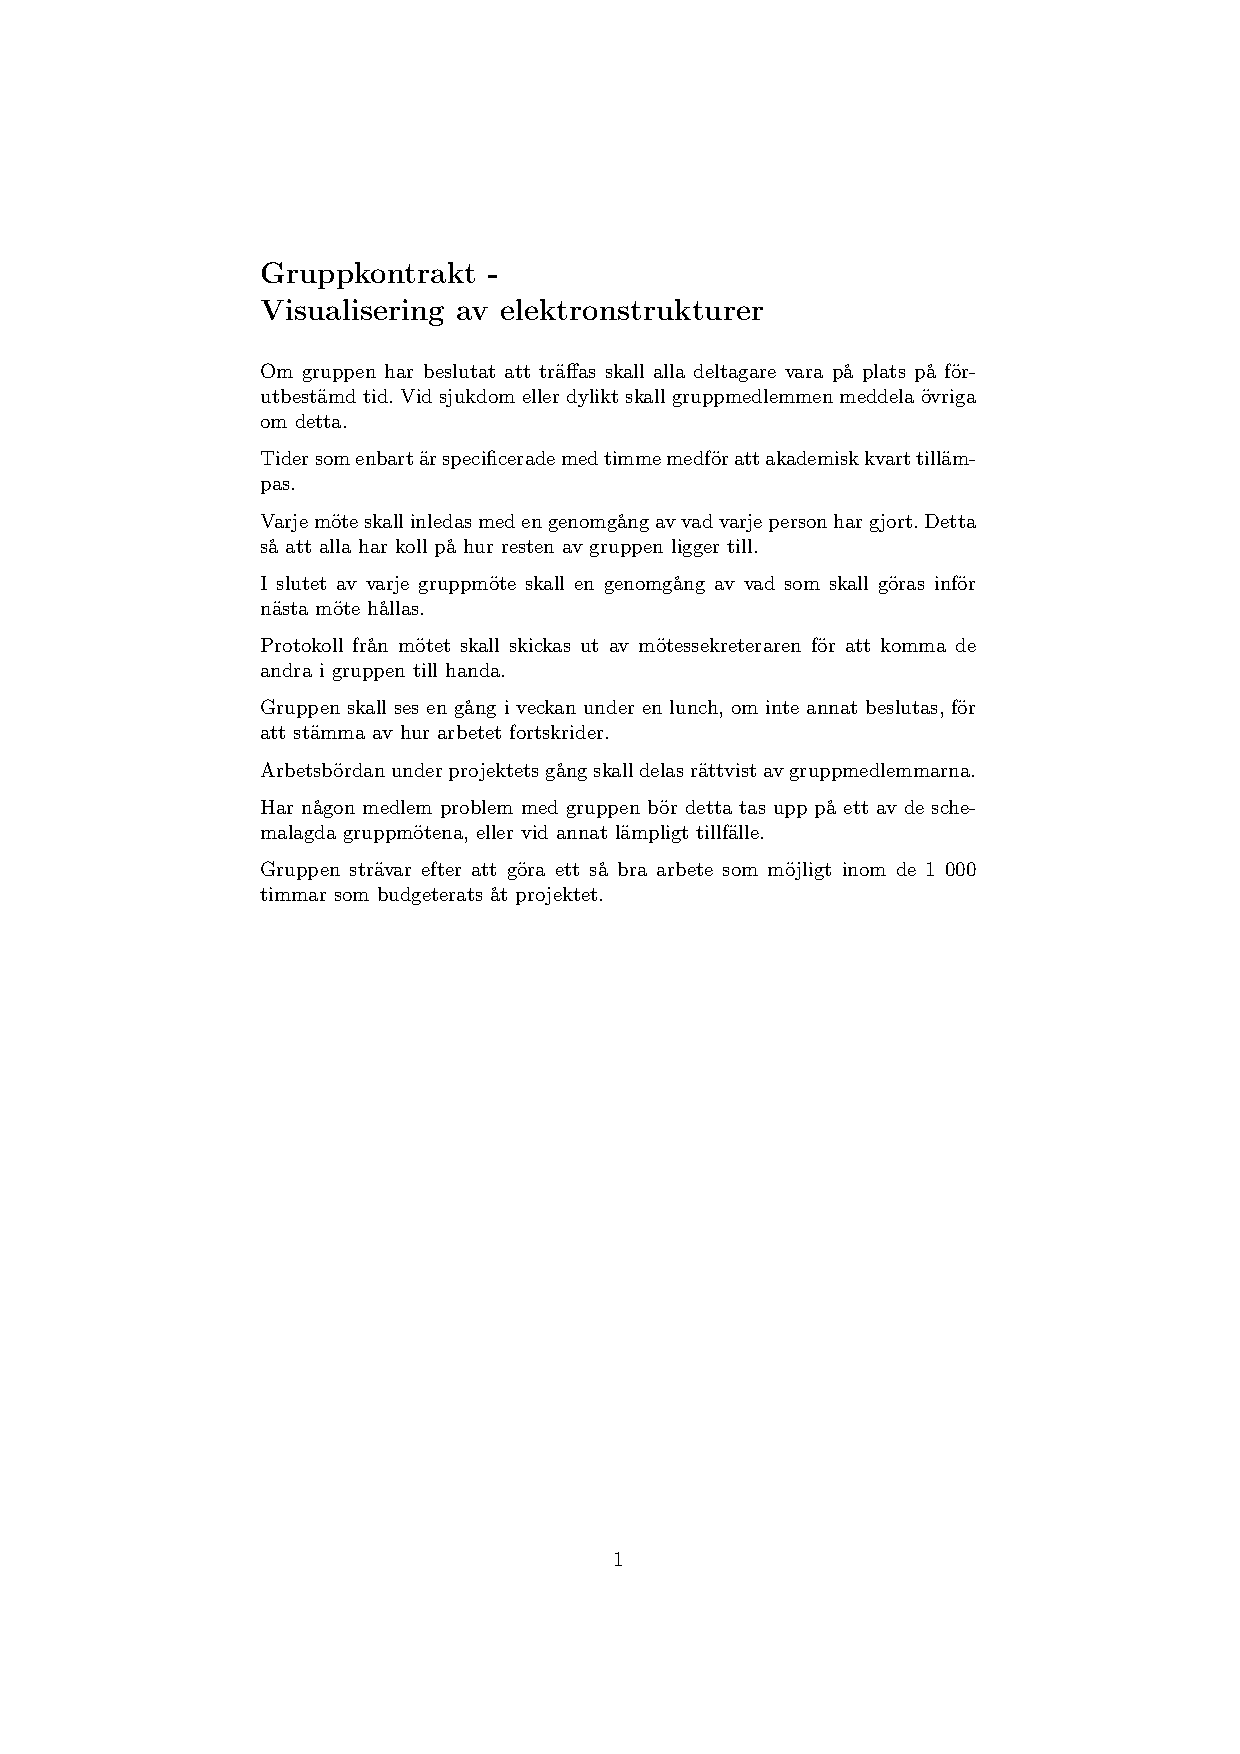
\includepdf[pages={1},pagecommand=\section{Gruppkontrakt}\label{appendix:Gruppkontrakt}\thispagestyle{empty}]{Gruppkontrakt.pdf}
	
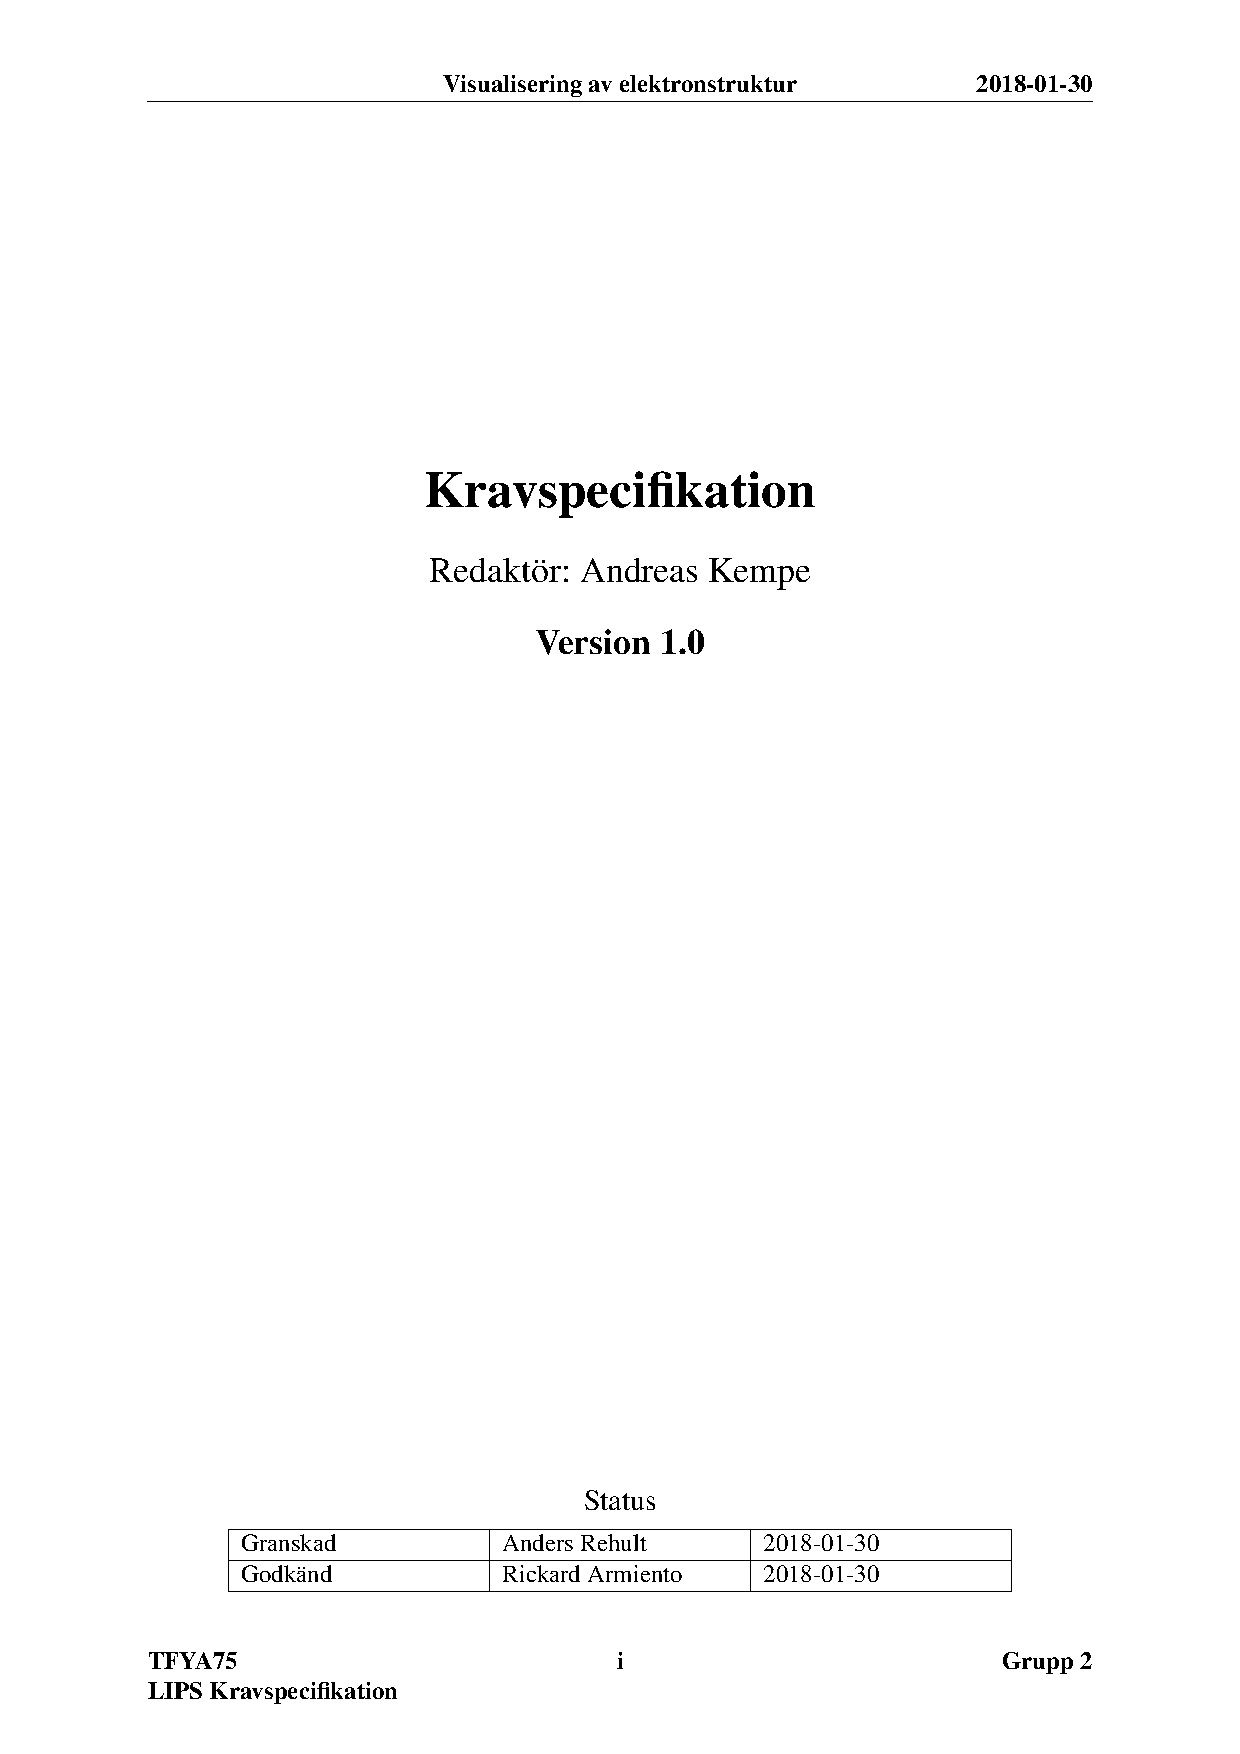
\includepdf[pages={1},pagecommand=\section{Kravspecifikation}\label{appendix:kravspecifikation}\thispagestyle{empty}]{Kravspecifikation_10.pdf}	\includepdf[pages={2-}]{Kravspecifikation_10.pdf}
	
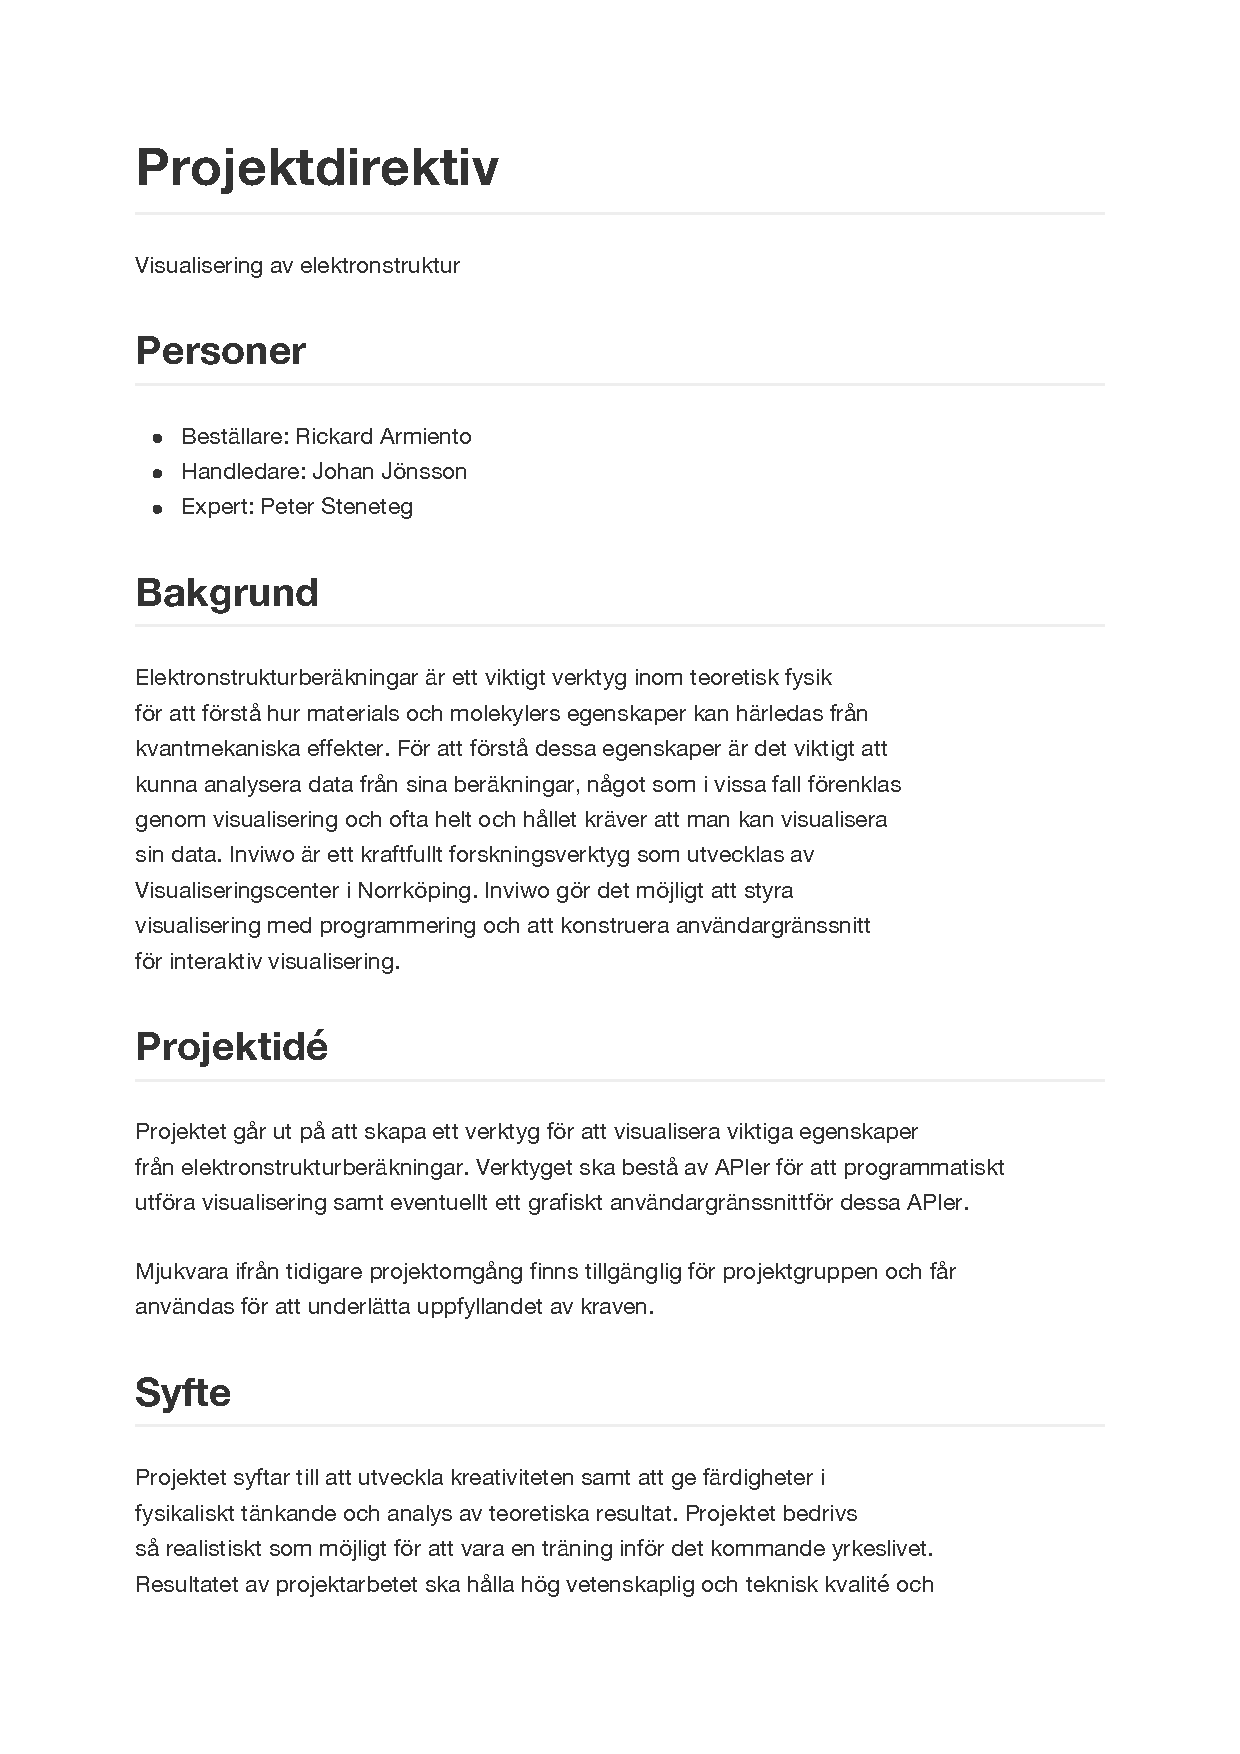
\includepdf[pages={1},pagecommand=\section{Projektdirektiv}\label{appendix:projektdirektiv}\thispagestyle{empty}]{projektdirektiv.pdf}
\includepdf[pages={2-}]{projektdirektiv.pdf}
	
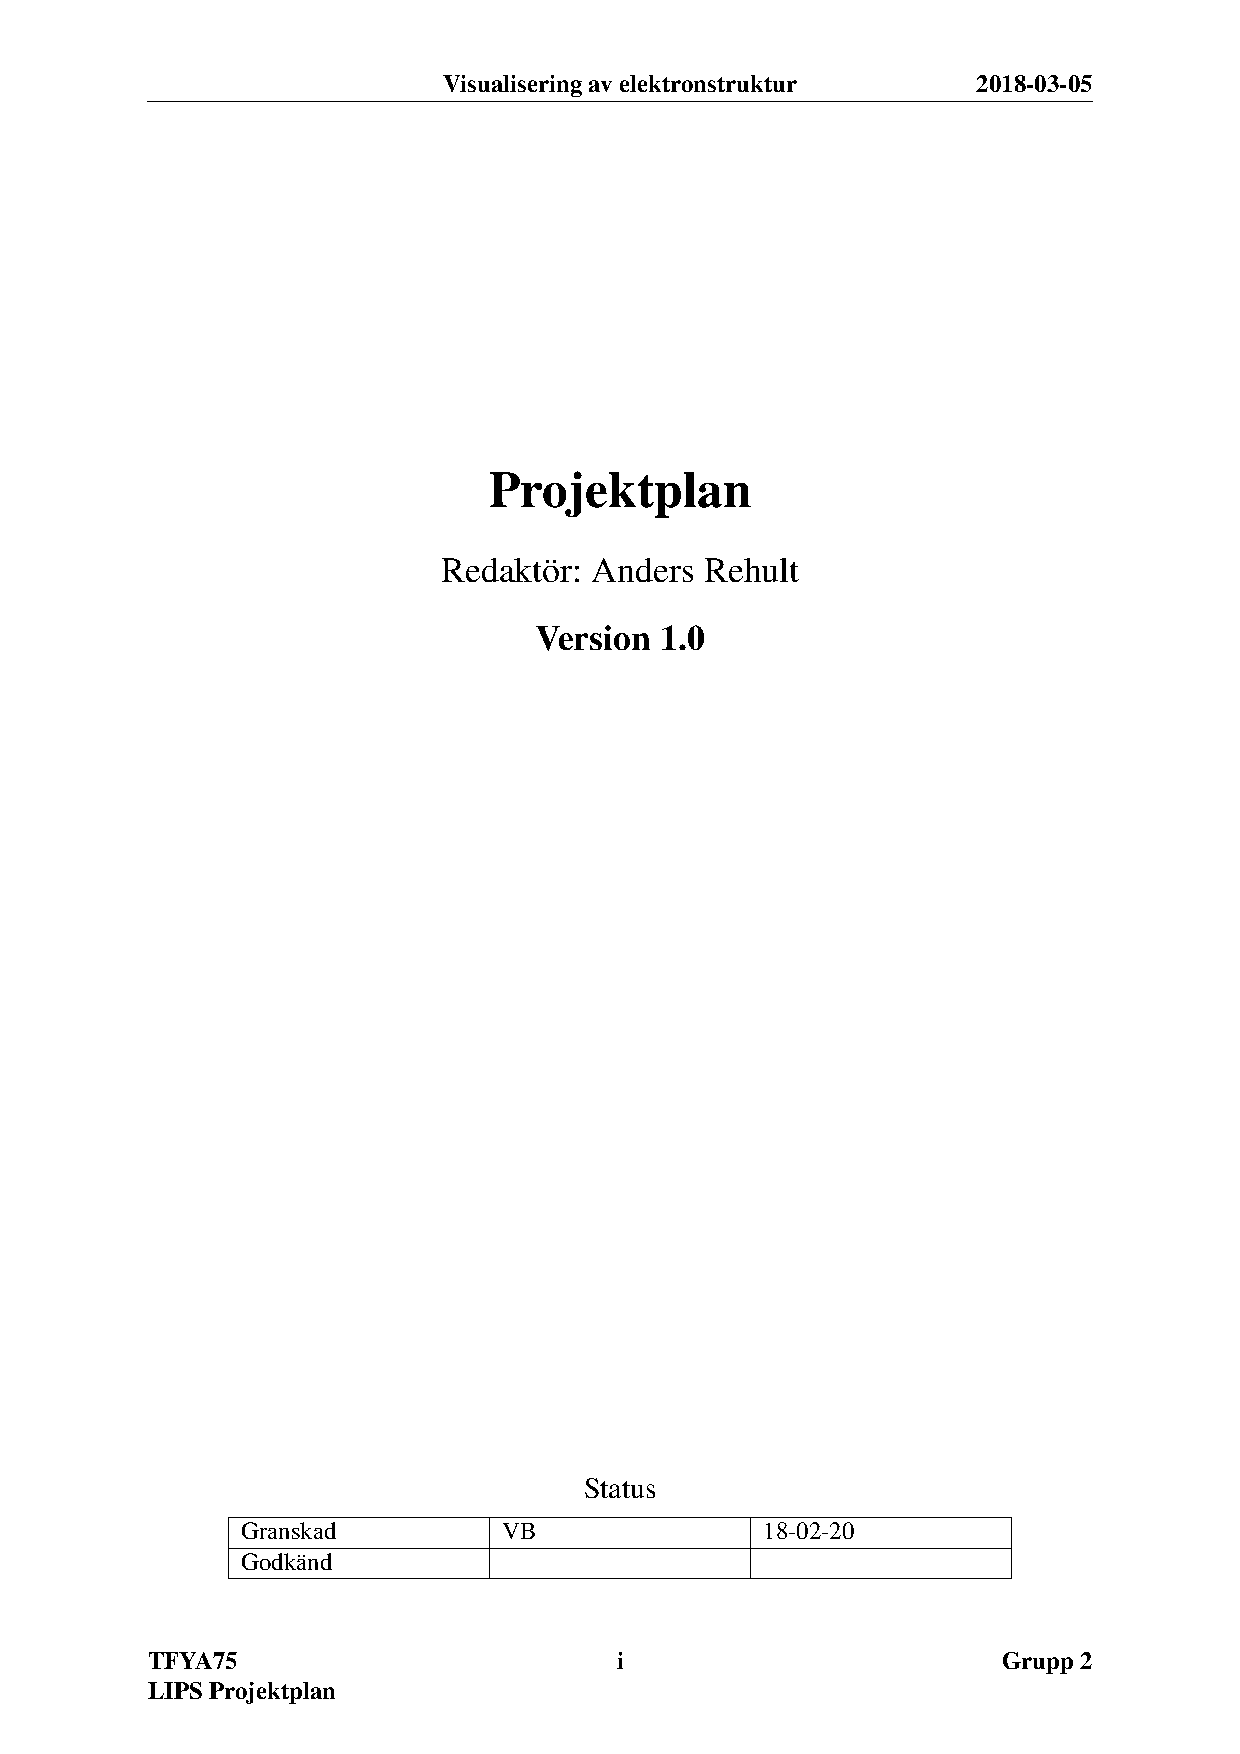
\includepdf[pages={1},pagecommand=\section{Projektplan}\label{appendix:projektplan}\thispagestyle{empty}]{projektplan_10.pdf}
\includepdf[pages={2-}]{projektplan_10.pdf}
	
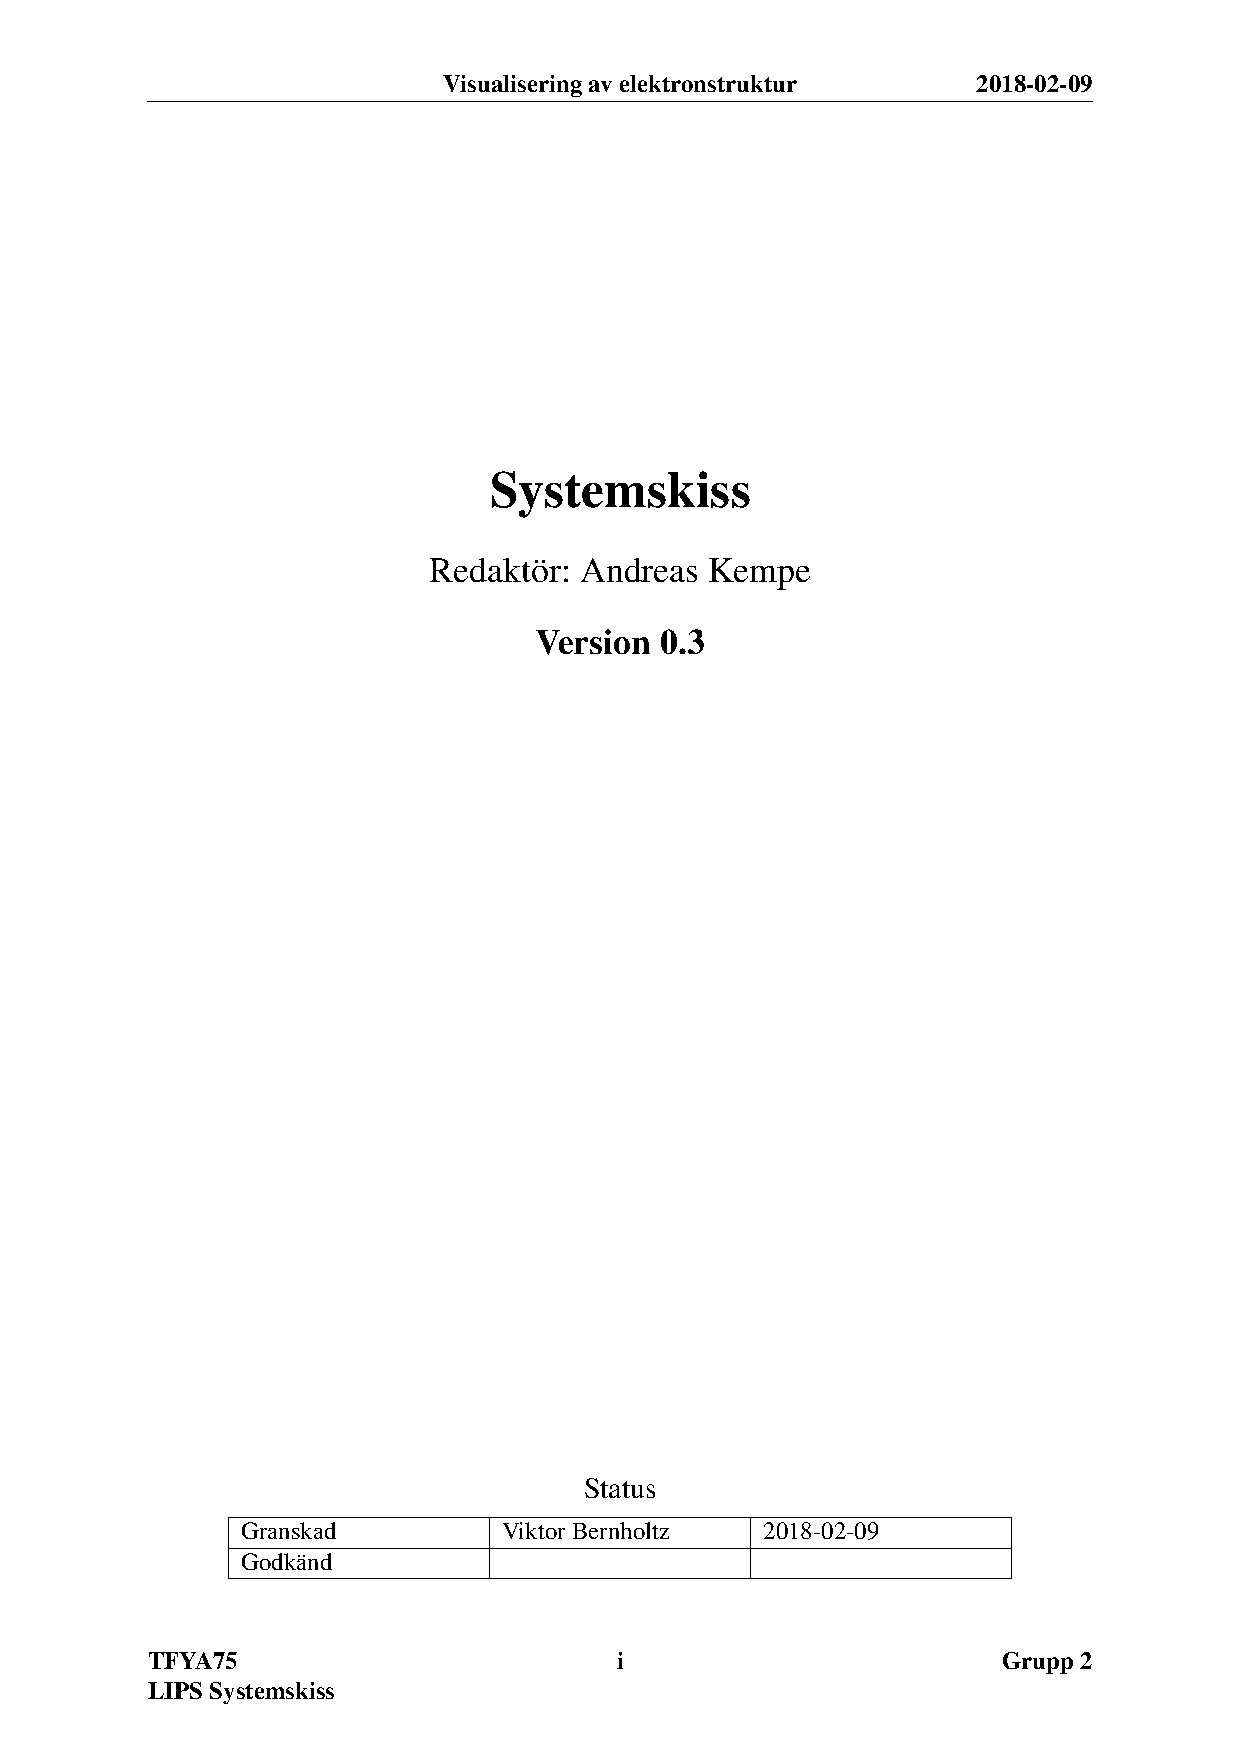
\includepdf[pages={1},pagecommand=\section{Systemskiss}\label{appendix:systemskiss}\thispagestyle{empty}]{Systemskiss_03.pdf}
\includepdf[pages={2-}]{Systemskiss_03.pdf}
	
	
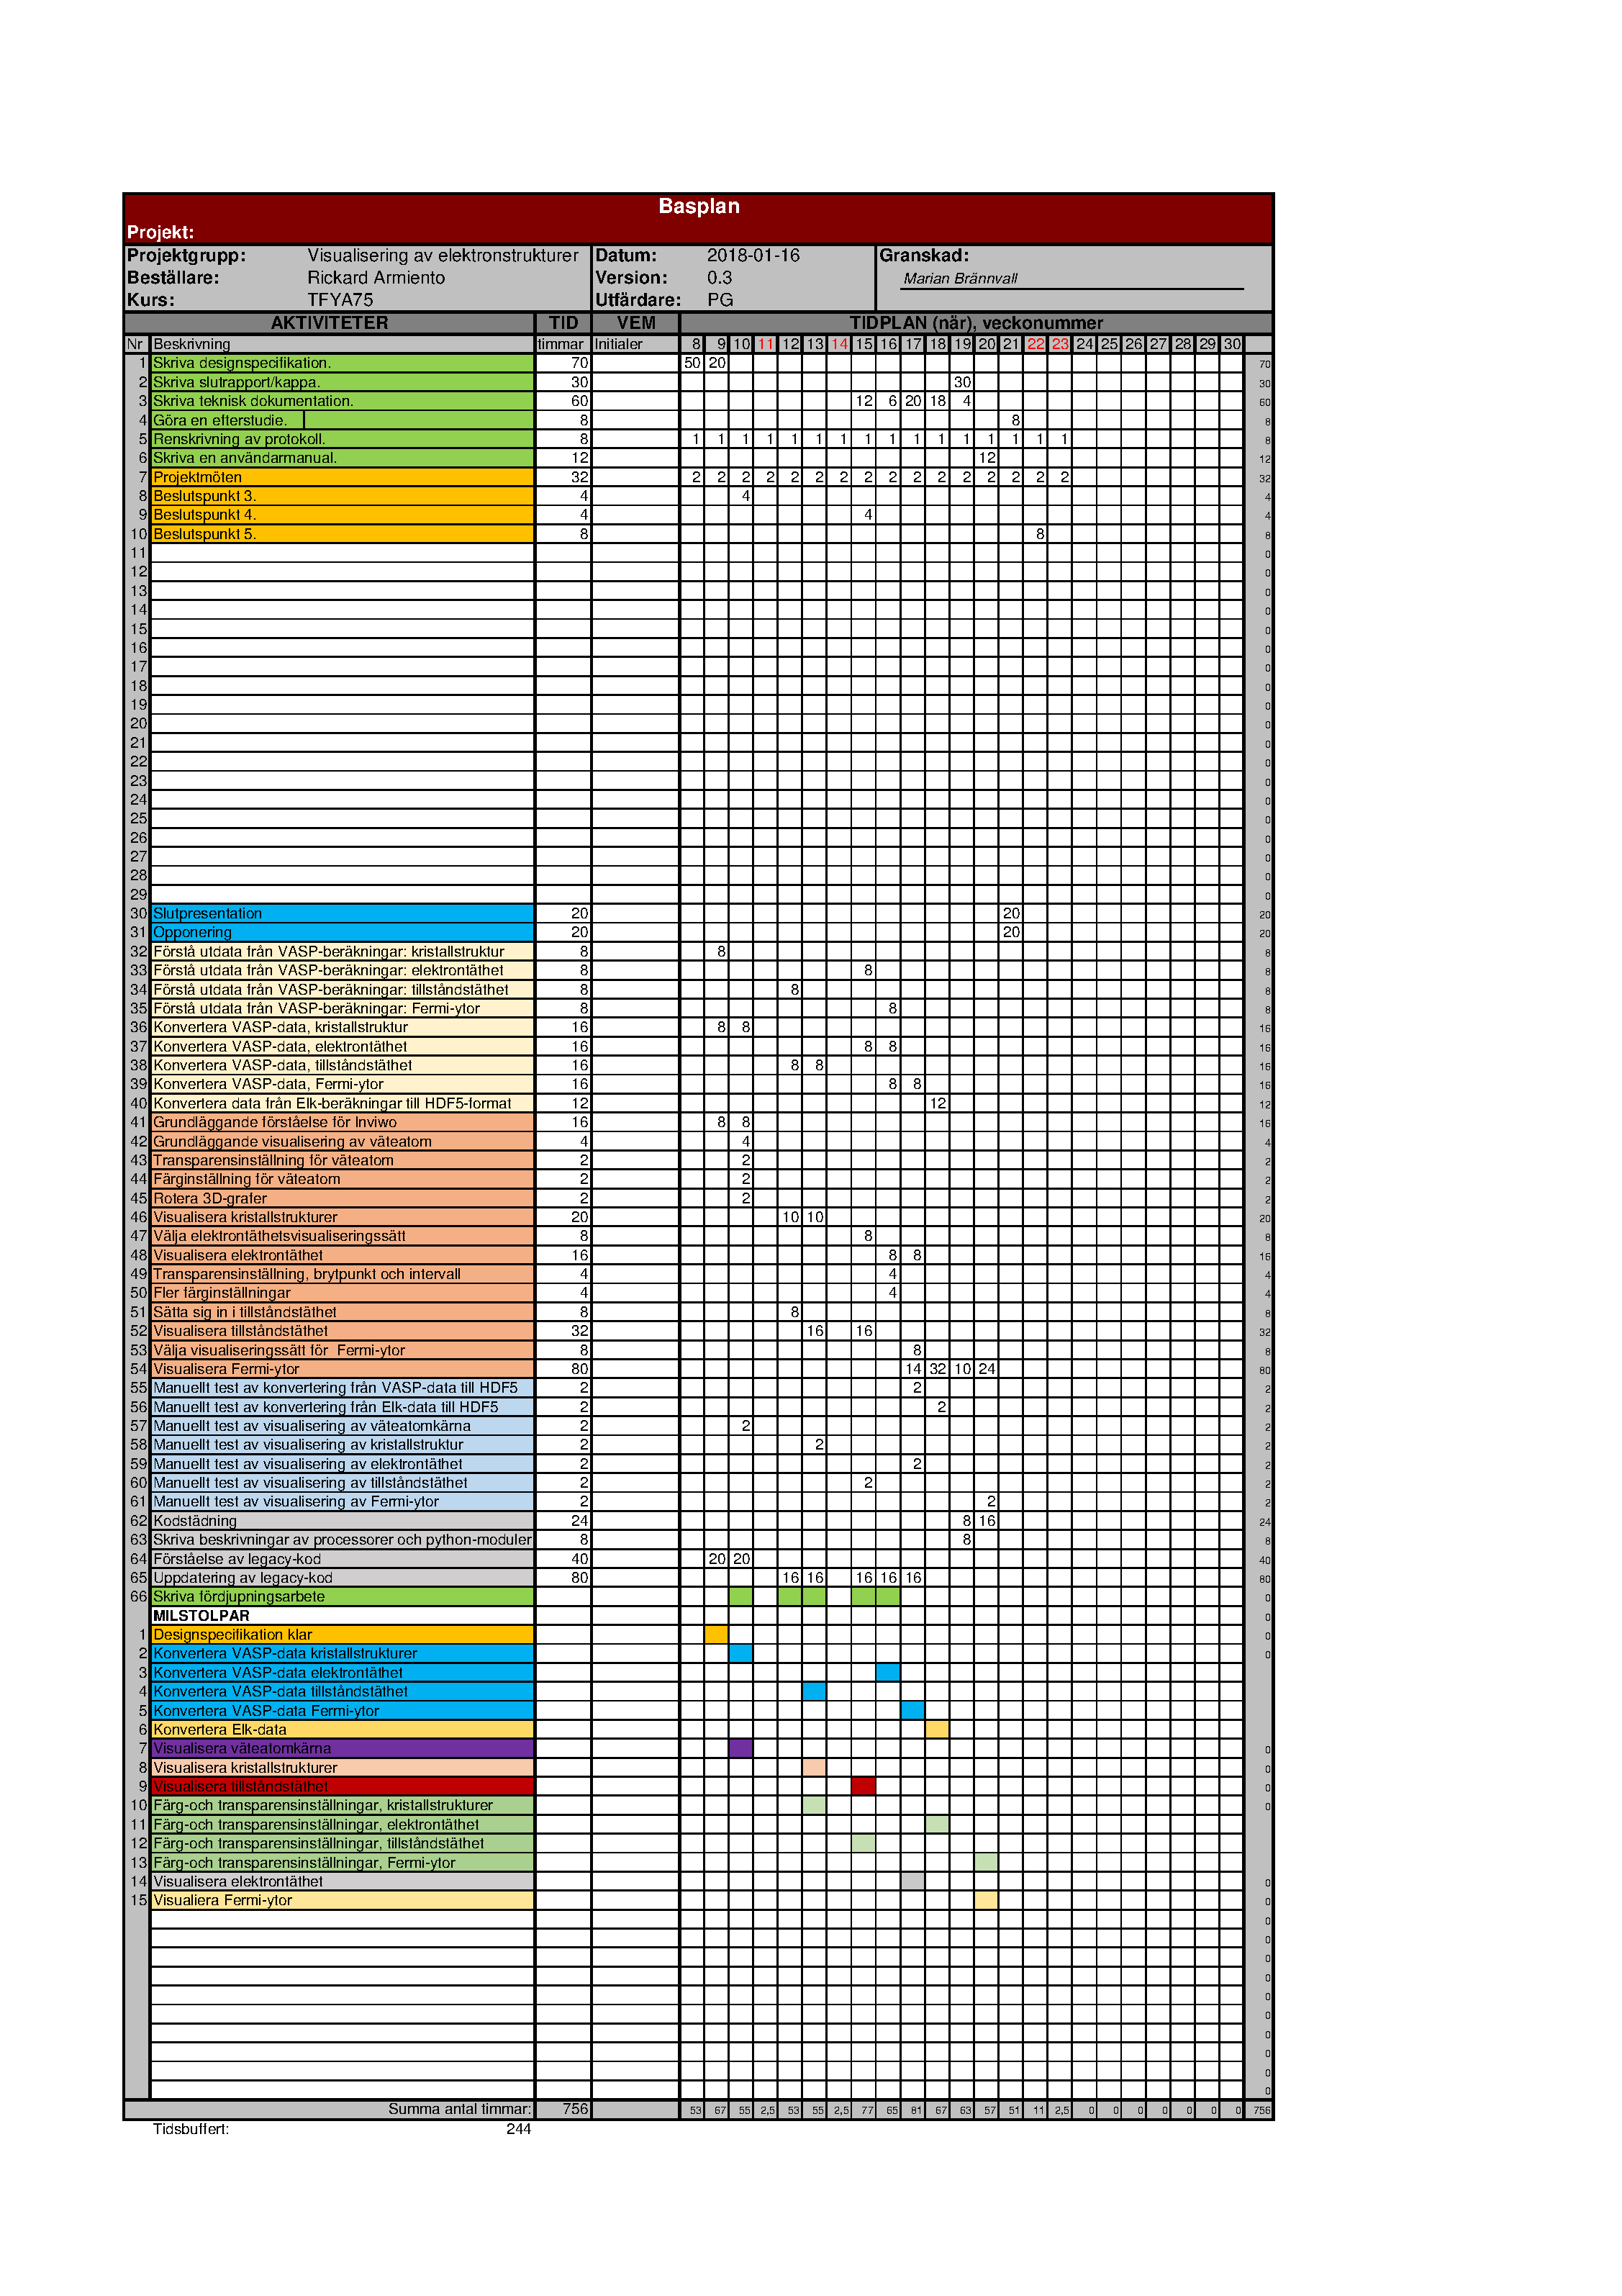
\includepdf[pages={1},pagecommand=\section{Tidplan}\label{appendix:tidplan}\thispagestyle{empty}]{tidplan_03.pdf}
	
	
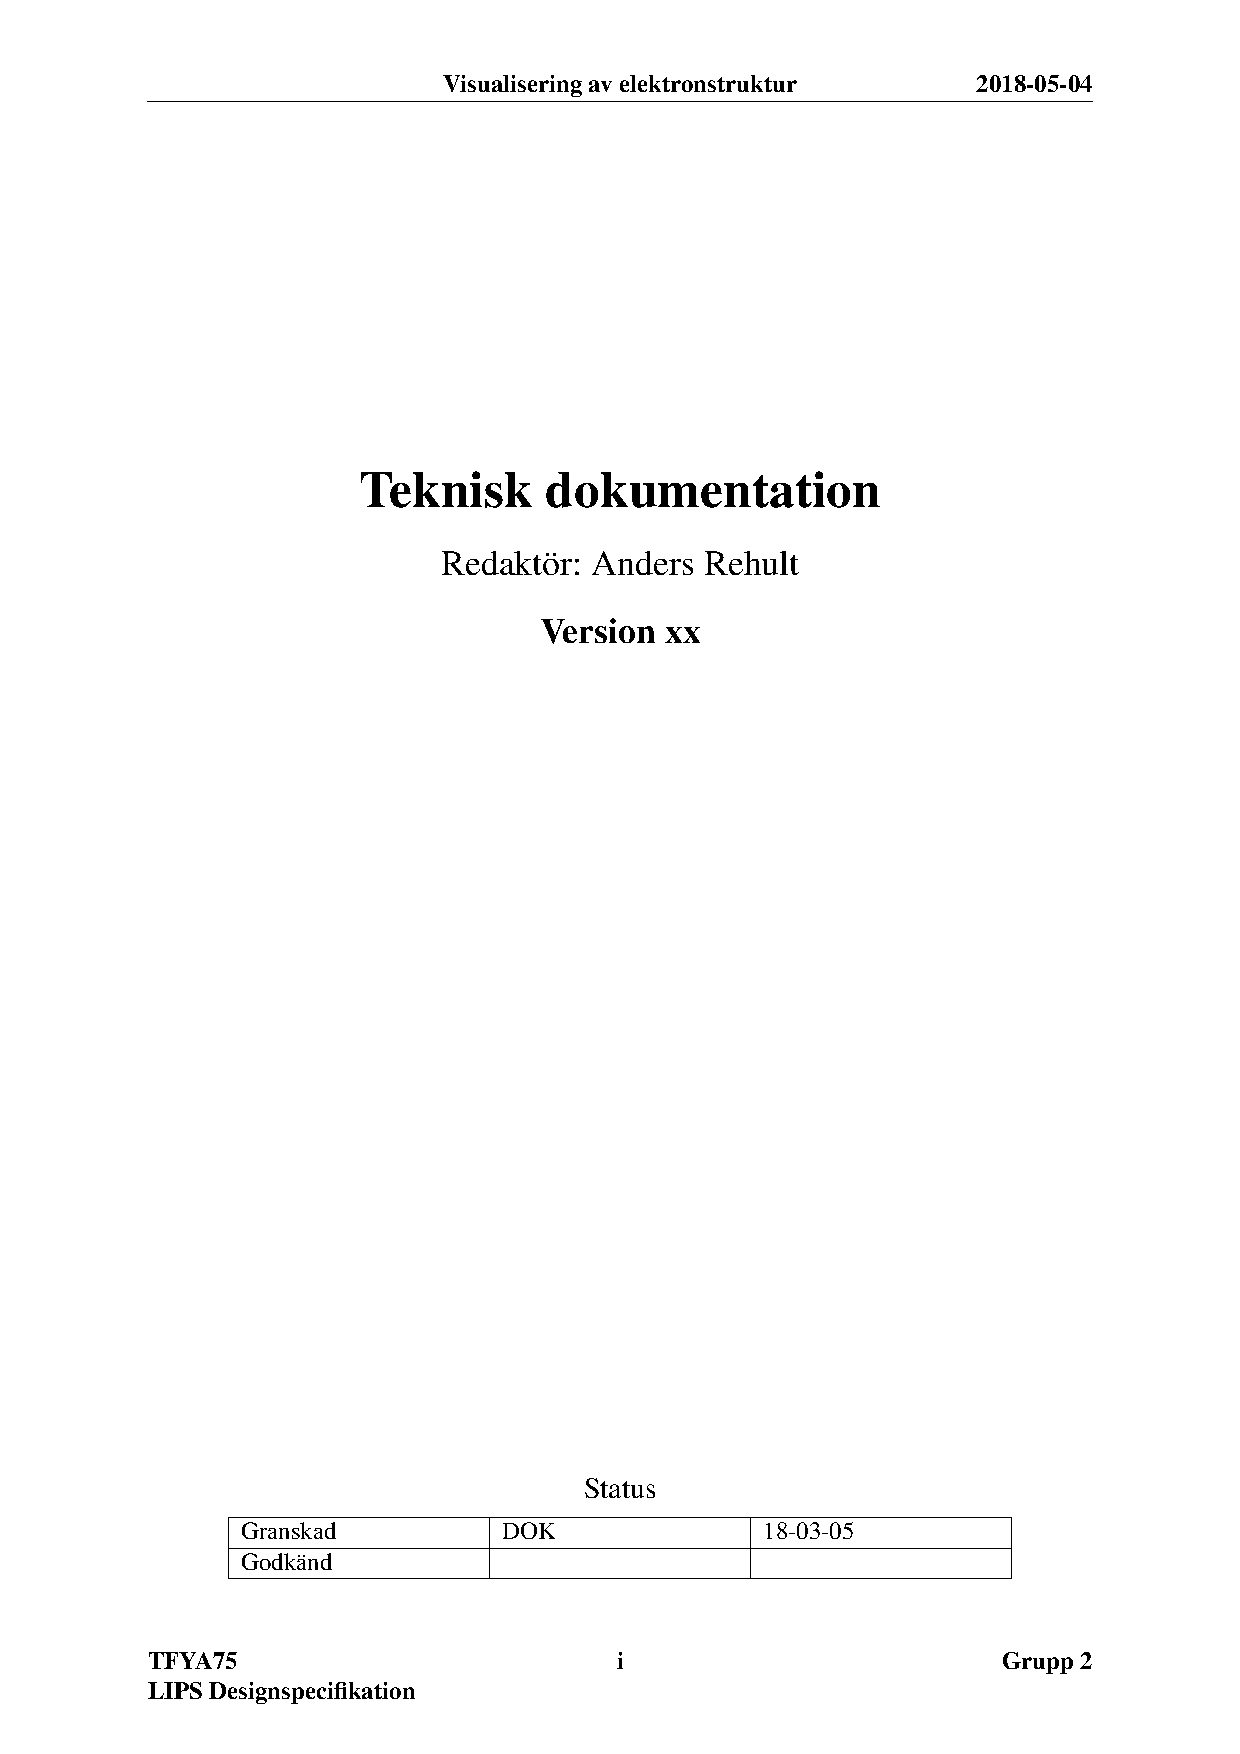
\includepdf[pages={1},pagecommand=\section{Teknisk dokumentation}\label{appendix:teknisk-dokumentation}\thispagestyle{empty}]{tekdok.pdf}
\includepdf[pages={2-}]{tekdok.pdf}

\end{appendices}

\end{document} 
